\newcommand{\packedTagResultsAucTable}{
    \begin{table}[H]
        \centering
        \begin{tabular}{|p{2,8cm}||p{2,8cm} p{2,8cm} p{2,8cm}|}
            \hline
            Packed Tag & ALOHA & Joint Embedding & Proposed Model \\
            \hline
            AUC-ROC & 0.978$\pm$0.001 & 0.978$\pm$0.003 & \textBF{0.981$\pm$0.001} \\
            \hline
        \end{tabular}
        \caption{AUC-ROC (Area Under Curve) of the different models for the \textbf{Packed Tag} prediction task. Results were aggregated over \textBF{3} training runs with different weight initializations and minibatch orderings. Best results are shown in \textbf{bold}.} \label{tab:packedTag_auc}
    \end{table}
}

\newcommand{\packedTagResultsAtFprTable}{
    \begin{center}
        \begin{longtable}[c]{|p{3,2cm}||p{1,8cm} p{1,8cm} p{1,8cm} p{1,8cm} p{1,8cm}|}
            \hline
            Packed Tag & \multicolumn{5}{c|}{{FPR}} \\
            & $10^{-5}$ & $10^{-4}$ & $10^{-3}$ & $10^{-2}$ & $10^{-1}$ \\
            \hline
            \endfirsthead

            \caption*{\raggedright ...continued from previous page} \\
            \hline
            Packed Tag & \multicolumn{5}{c|}{\textbf{FPR}} \\
            & $10^{-5}$ & $10^{-4}$ & $10^{-3}$ & $10^{-2}$ & $10^{-1}$ \\
            \hline
            \endhead

            \caption*{\raggedleft ...continued on next page} \\
            \endfoot

            \caption{Mean and standard deviation results (TPR, Accuracy, Recall, Precision and F1-Score) of the different models for the \textbf{Packed Tag} prediction task at different \textbf{FPR}s (\textit{False Positive Rates}). Results were aggregated over \textBF{3} training runs with different weight initializations and minibatch orderings. Best results are shown in \textbf{bold}. Under \textbf{TPR} results are also presented the percentage reduction in mean detection error and in ROC curve standard deviation introduced by the \textit{Proposed Model} with respect to both \textit{ALOHA} model and \textit{Joint Embedding}.} \label{tab:packedTag_results_at_fpr} \\
            \endlastfoot

            \multicolumn{6}{|c|}{\textbf{TPR}} \\
            \hline
            ALOHA & 0.011$\pm$0.013 & 0.223$\pm$0.134 & 0.593$\pm$0.013 & 0.675$\pm$0.017 & 0.945$\pm$0.005 \\
            Joint Embedding & 0.003$\pm$0.003 & 0.224$\pm$0.057 & \textBF{0.611$\pm$0.016} & 0.731$\pm$0.019 & 0.939$\pm$0.010 \\
            Proposed Model & \textBF{0.059$\pm$0.037} & \textBF{0.315$\pm$0.069} & 0.543$\pm$0.119 & \textBF{0.743$\pm$0.027} & \textBF{0.950$\pm$0.003} \\
            \hline
            Error Reduction wrt \newline ALOHA & 4.9\% & 11.8\% & -12.3\% & 20.9\% & 9.1\% \\
            Error Reduction wrt \newline Joint Embedding & 5.6\% & 11.7\% & -17.5\% & 4.5\% & 18.0\% \\
            \hline
            Std Reduction wrt \newline ALOHA & -184.6\% & 48.5\% & -815.4\% & -58.8\% & 40.0\% \\
            Std Reduction wrt \newline Joint Embedding & -1133.3\% & -21.1\% & -643.7\% & -42.1\% & 70.0\% \\
            \hline
            \multicolumn{6}{|c|}{\textbf{Accuracy}} \\
            \hline
            ALOHA & 0.865$\pm$0.002 & 0.894$\pm$0.018 & 0.944$\pm$0.002 & 0.947$\pm$0.002 & 0.906$\pm$0.001 \\
            Joint Embedding & 0.864$\pm$0.000 & 0.894$\pm$0.008 & \textBF{0.946$\pm$0.002} & 0.955$\pm$0.003 & 0.905$\pm$0.001 \\
            Proposed Model & \textBF{0.872$\pm$0.005} & \textBF{0.906$\pm$0.009} & 0.937$\pm$0.016 & \textBF{0.956$\pm$0.004} & \textBF{0.907$\pm$0.000} \\
            \hline
            \multicolumn{6}{|c|}{\textbf{Recall}} \\
            \hline
            ALOHA & 0.011$\pm$0.013 & 0.223$\pm$0.134 & 0.593$\pm$0.013 & 0.675$\pm$0.017 & 0.945$\pm$0.005 \\
            Joint Embedding & 0.003$\pm$0.003 & 0.224$\pm$0.057 & \textBF{0.611$\pm$0.016} & 0.731$\pm$0.019 & 0.939$\pm$0.010 \\
            Proposed Model & \textBF{0.059$\pm$0.037} & \textBF{0.315$\pm$0.069} & 0.543$\pm$0.119 & \textBF{0.743$\pm$0.027} & \textBF{0.950$\pm$0.003} \\
            \hline
            \multicolumn{6}{|c|}{\textbf{Precision}} \\
            \hline
            ALOHA & 0.986$\pm$0.013 & 0.992$\pm$0.008 & 0.989$\pm$0.000 & 0.914$\pm$0.002 & 0.599$\pm$0.001 \\
            Joint Embedding & 0.998$\pm$0.002 & 0.997$\pm$0.001 & \textBF{0.990$\pm$0.000} & 0.920$\pm$0.002 & 0.598$\pm$0.003 \\
            Proposed Model & \textBF{0.999$\pm$0.000} & \textBF{0.998$\pm$0.000} & 0.988$\pm$0.003 & \textBF{0.921$\pm$0.003} & \textBF{0.600$\pm$0.001} \\
            \hline
            \multicolumn{6}{|c|}{\textbf{F1 Score}} \\
            \hline
            ALOHA & 0.022$\pm$0.025 & 0.343$\pm$0.197 & 0.741$\pm$0.010 & 0.776$\pm$0.012 & 0.733$\pm$0.003 \\
            Joint Embedding & 0.005$\pm$0.006 & 0.362$\pm$0.073 & \textBF{0.756$\pm$0.012} & 0.815$\pm$0.012 & 0.730$\pm$0.005 \\
            Proposed Model & \textBF{0.109$\pm$0.065} & \textBF{0.475$\pm$0.077} & 0.692$\pm$0.106 & \textBF{0.822$\pm$0.018} & \textBF{0.736$\pm$0.001} \\
            \hline
        \end{longtable}
    \end{center}
}

\newcommand{\packedTagResultsSummaryTable}{
    \begin{table}[H]
        \centering
        \begin{tabular}{|p{3,2cm}||p{1,8cm} p{1,8cm} p{1,8cm} p{1,8cm} p{1,8cm}|}
            \hline
            \multicolumn{6}{|c|}{Packed Tag (at FPR $=1\%$)} \\
            \hline
            Model & TPR & Accuracy & Precision & Recall & F1 score \\
            \hline
            ALOHA & 0.675$\pm$0.017 & 0.947$\pm$0.002 & 0.914$\pm$0.002 & 0.675$\pm$0.017 & 0.776$\pm$0.012 \\
            Joint Embedding & 0.731$\pm$0.019 & 0.955$\pm$0.003 & 0.920$\pm$0.002 & 0.731$\pm$0.019 & 0.815$\pm$0.012 \\
            Proposed Model & \textBF{0.743$\pm$0.027} & \textBF{0.956$\pm$0.004} & \textBF{0.921$\pm$0.003} & \textBF{0.743$\pm$0.027} & \textBF{0.822$\pm$0.018} \\
            \hline
        \end{tabular}
        \caption{Summary of the mean and standard deviation results of the different models for the \textbf{Packed Tag} prediction task at \textbf{FPR} $=1\%$. Results were aggregated over \textBF{3} training runs with different weight initializations and minibatch orderings. Best results are shown in \textbf{bold}.} \label{tab:packedTag_result_summary}
    \end{table}
}

\newcommand{\packedTagRocAloha}{
    \begin{figure}[H]
        \vspace*{-0.5cm}
        \centering
        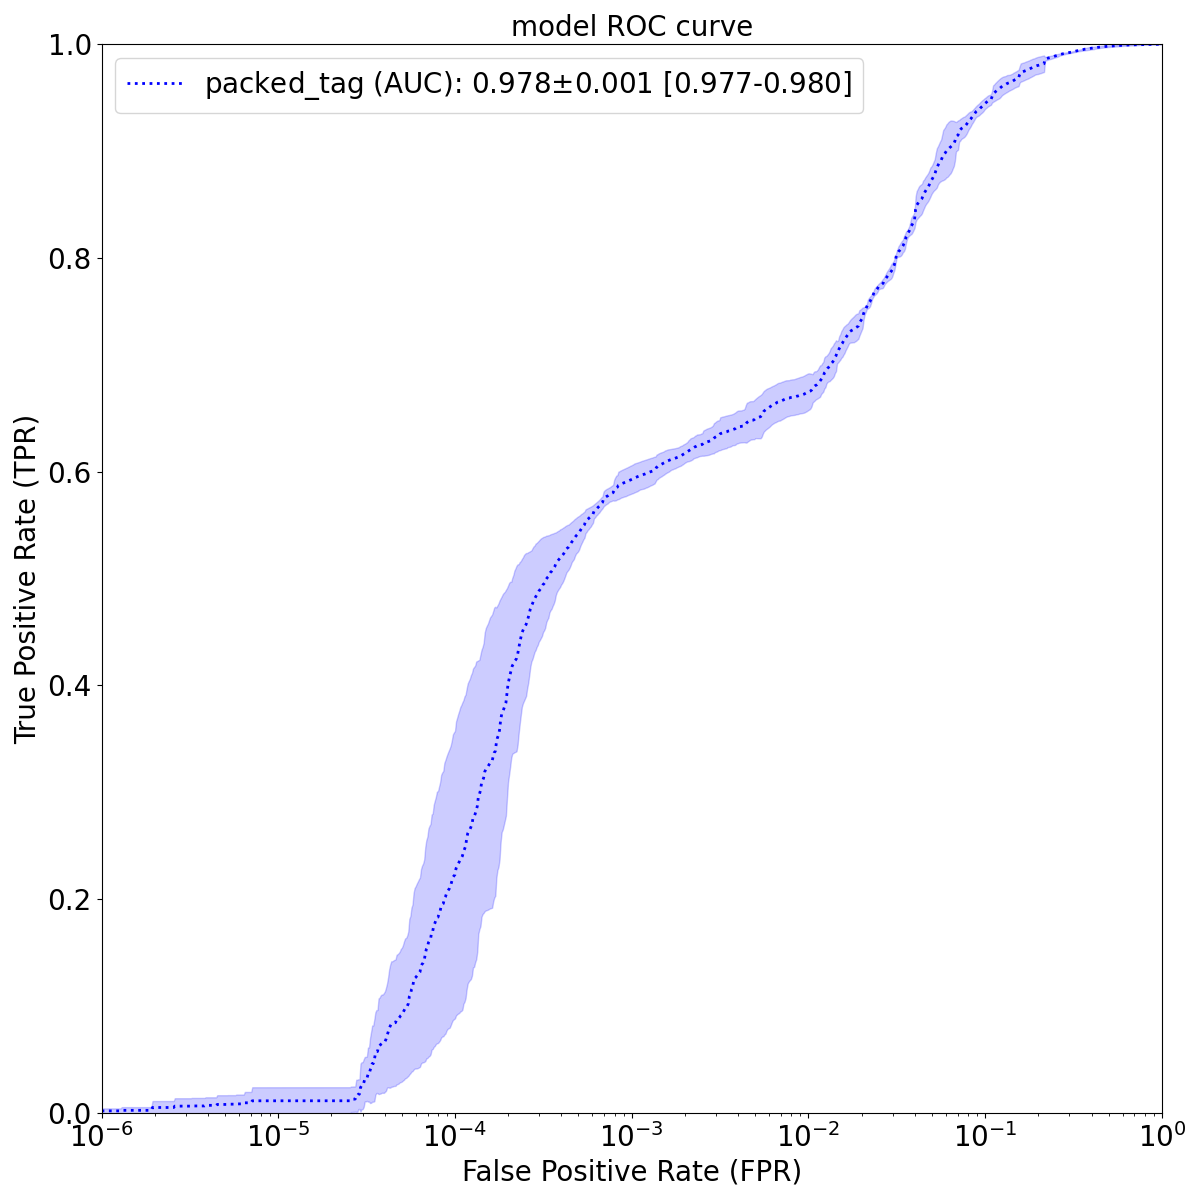
\includegraphics[width=0.6\textwidth]{./results/packed_tag_roc_aloha.png}
        \vspace*{-0.2cm}
        \caption{ROC curve and AUC statistics of \textBF{ALOHA} model for the \textbf{Packed Tag}. The line represents the \textit{mean} TPR at a given FPR, while the shaded region represents the \textit{standard deviation}. Statistics were computed over \textBF{3} training runs, each with random parameter initialization.}
        \label{fig:packedTagRocAloha}
    \end{figure}
}

\newcommand{\packedTagRocJointEmbedding}{
    \begin{figure}[H]
        \vspace*{-0.5cm}
        \centering
        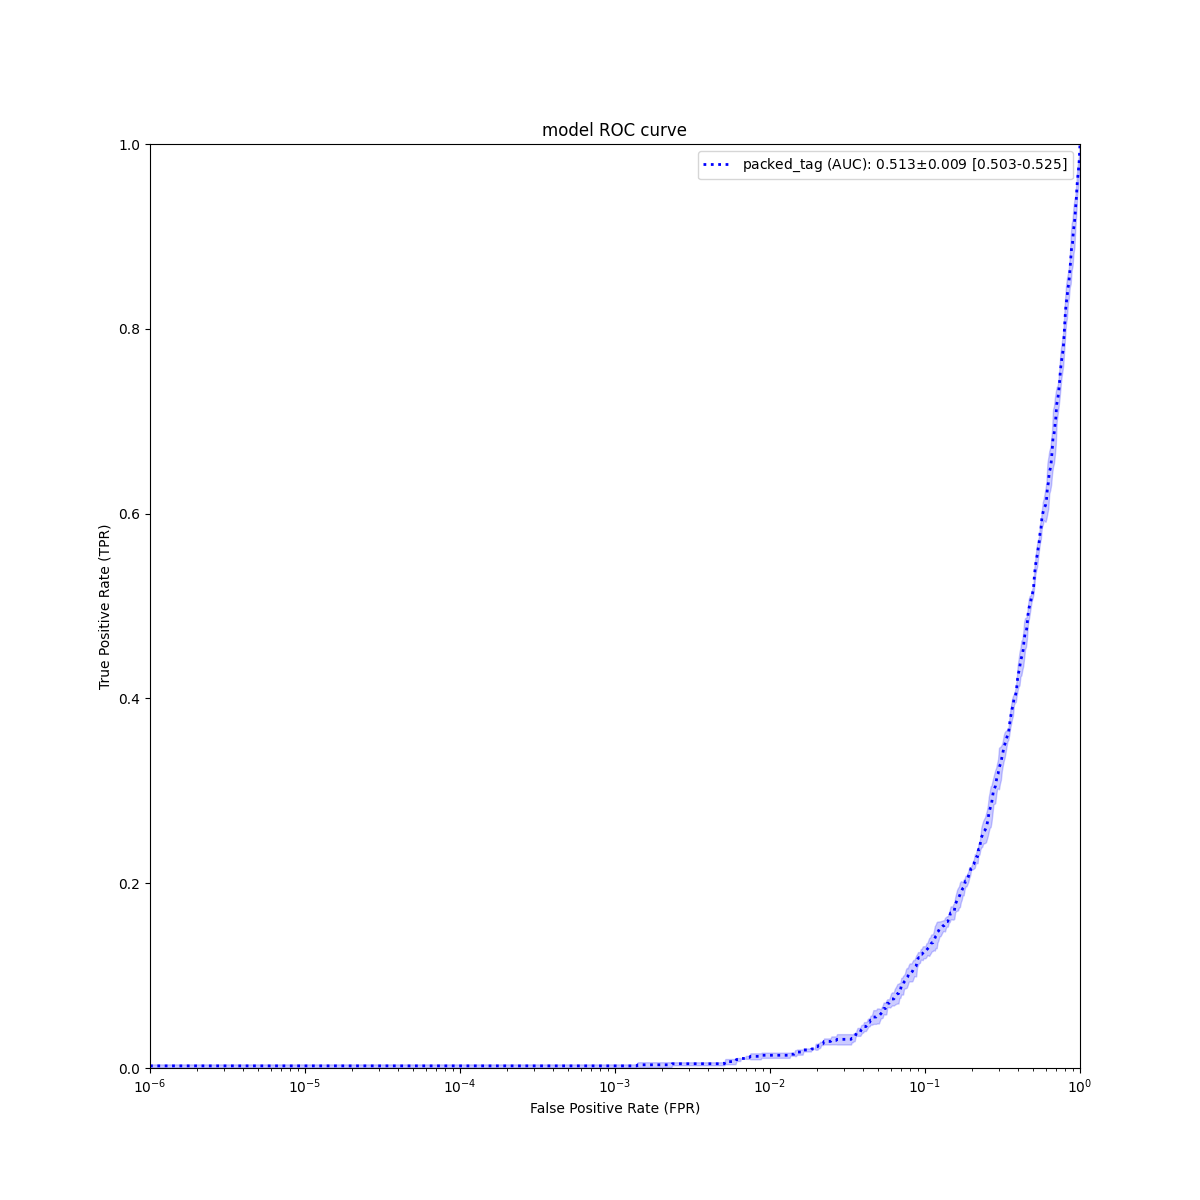
\includegraphics[width=0.6\textwidth]{./results/packed_tag_roc_jointEmbedding.png}
        \vspace*{-0.2cm}
        \caption{ROC curve and AUC statistics of \textBF{Joint Embedding} model for the \textbf{Packed Tag}. The line represents the \textit{mean} TPR at a given FPR, while the shaded region represents the \textit{standard deviation}. Statistics were computed over \textBF{3} training runs, each with random parameter initialization.}
        \label{fig:packedTagRocJointEmbedding}
    \end{figure}
}

\newcommand{\packedTagRocProposedMethod}{
    \begin{figure}[H]
        \vspace*{-0.5cm}
        \centering
        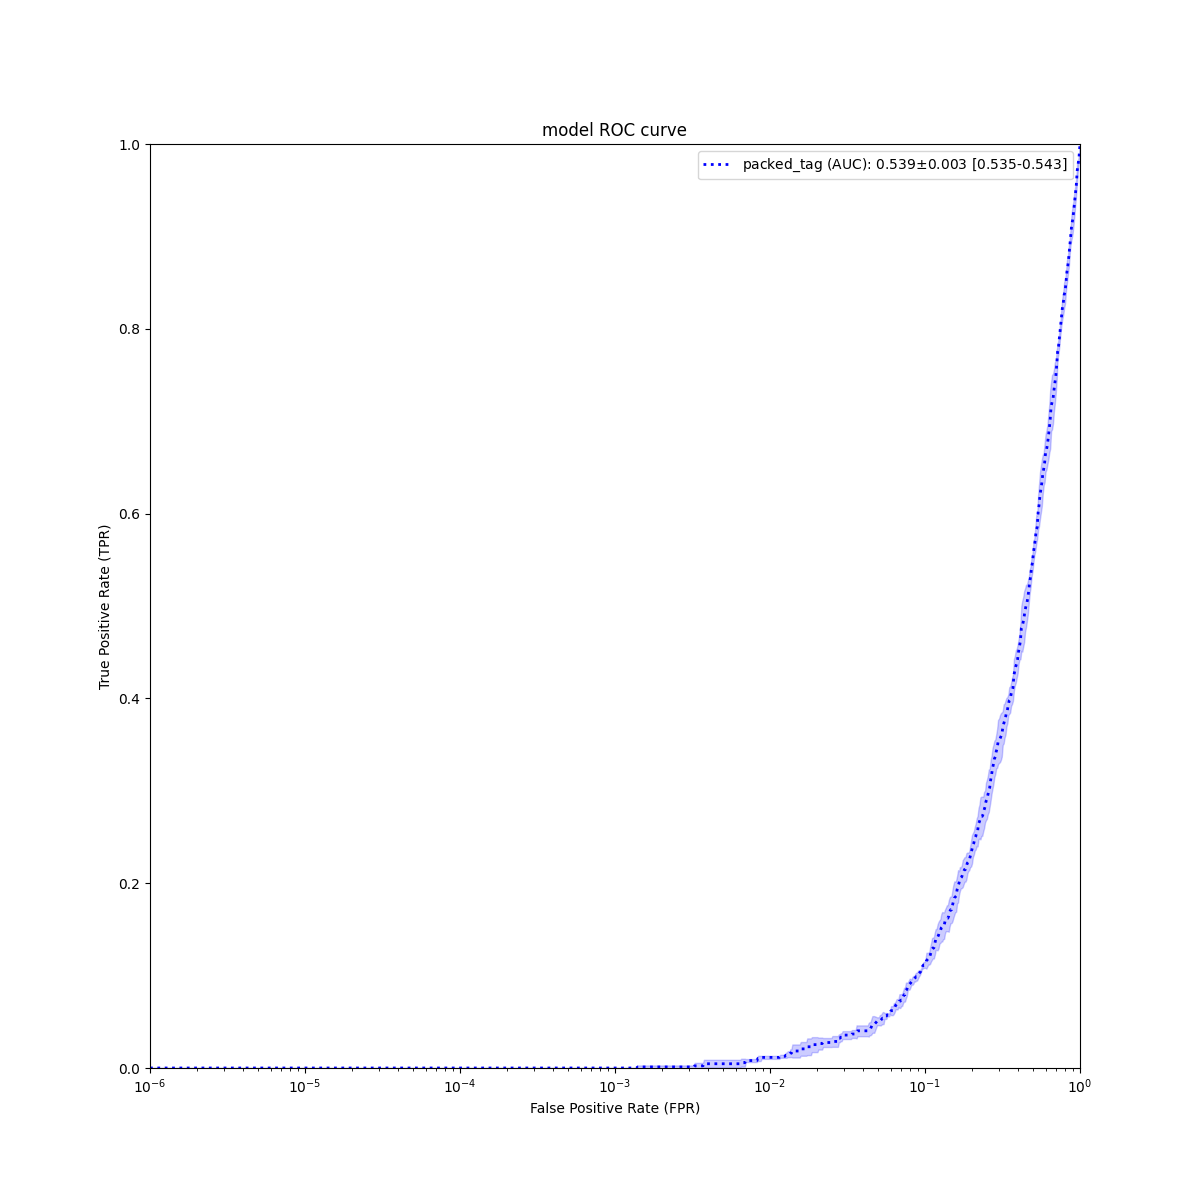
\includegraphics[width=0.6\textwidth]{./results/packed_tag_roc_proposedModel.png}
        \vspace*{-0.2cm}
        \caption{ROC curve and AUC statistics of \textBF{Proposed Model} for the \textbf{Packed Tag}. The line represents the \textit{mean} TPR at a given FPR, while the shaded region represents the \textit{standard deviation}. Statistics were computed over \textBF{3} training runs, each with random parameter initialization.}
        \label{fig:packedTagRocProposedModel}
    \end{figure}
}
